\documentclass[paper=a4, fontsize=11pt]{scrartcl} % A4 paper and 11pt font size

\usepackage[T1]{fontenc} % Use 8-bit encoding that has 256 glyphs
\usepackage[english]{babel} % English language/hyphenation
\usepackage{amsmath,amsfonts,amsthm} % Math packages
\usepackage{graphicx}

\usepackage{lipsum} % Used for inserting dummy 'Lorem ipsum' text into the template

\usepackage{sectsty} % Allows customizing section commands
\allsectionsfont{\centering \normalfont\scshape} % Make all sections centered, the default font and small caps

\usepackage{fancyhdr} % Custom headers and footers
\pagestyle{fancyplain} % Makes all pages in the document conform to the custom headers and footers
\fancyhead{} % No page header - if you want one, create it in the same way as the footers below
\fancyfoot[L]{} % Empty left footer
\fancyfoot[C]{} % Empty center footer
\fancyfoot[R]{\thepage} % Page numbering for right footer
\renewcommand{\headrulewidth}{0pt} % Remove header underlines
\renewcommand{\footrulewidth}{0pt} % Remove footer underlines
\setlength{\headheight}{13.6pt} % Customize the height of the header

\numberwithin{equation}{section} % Number equations within sections (i.e. 1.1, 1.2, 2.1, 2.2 instead of 1, 2, 3, 4)
\numberwithin{figure}{section} % Number figures within sections (i.e. 1.1, 1.2, 2.1, 2.2 instead of 1, 2, 3, 4)
\numberwithin{table}{section} % Number tables within sections (i.e. 1.1, 1.2, 2.1, 2.2 instead of 1, 2, 3, 4)

\setlength\parindent{0pt} % Removes all indentation from paragraphs - comment this line for an assignment with lots of text

%----------------------------------------------------------------------------------------
%	TITLE SECTION
%----------------------------------------------------------------------------------------

\newcommand{\horrule}[1]{\rule{\linewidth}{#1}} % Create horizontal rule command with 1 argument of height

\title{	
	\normalfont \normalsize 
	\textsc{EC500 - Introduction to Learning From Data} \\ [25pt] % Your university, school and/or department name(s)
	\horrule{0.5pt} \\[0.4cm] % Thin top horizontal rule
	\huge Matlab 4 \\ % The assignment title
	\horrule{2pt} \\[0.5cm] % Thick bottom horizontal rule
}

\author{Mikhail Andreev} % Your name

\date{\normalsize\today} % Today's date or a custom date

\begin{document}
	
	\maketitle % Print the title
	

	%----------------------------------------------------------------------------------------
	%	PROBLEM 1
	%----------------------------------------------------------------------------------------
	
	\newpage
	\section{k-Means vs. Spectral Clustering}
	The k-means approach to the dataset yield the following three graphs for k=2,3,4 respectively:\\\\\\
	\hspace*{-3cm}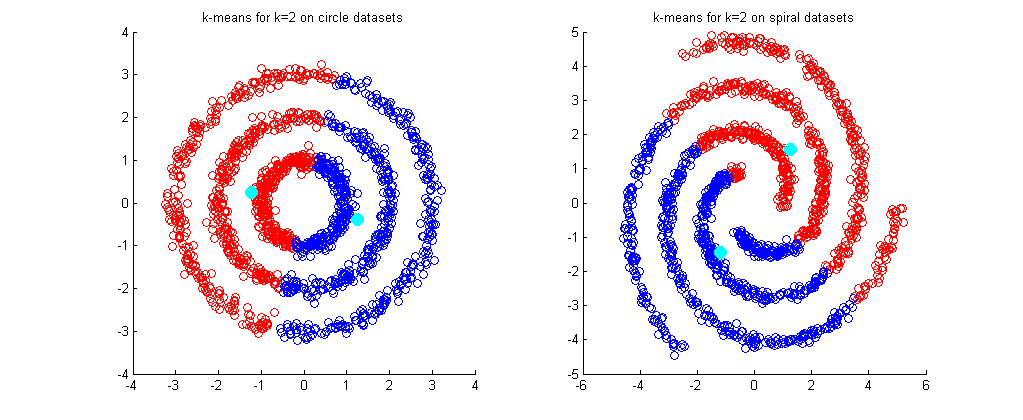
\includegraphics[scale=0.6]{kmeans_k2}
	\\\\\\
	\hspace*{-2.5cm}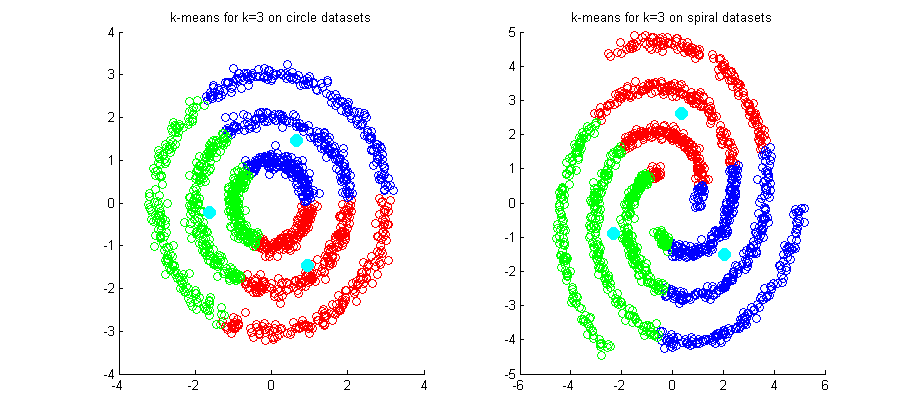
\includegraphics[scale=0.6]{kmeans_k3}
	\\\\\\
	\hspace*{-2.5cm}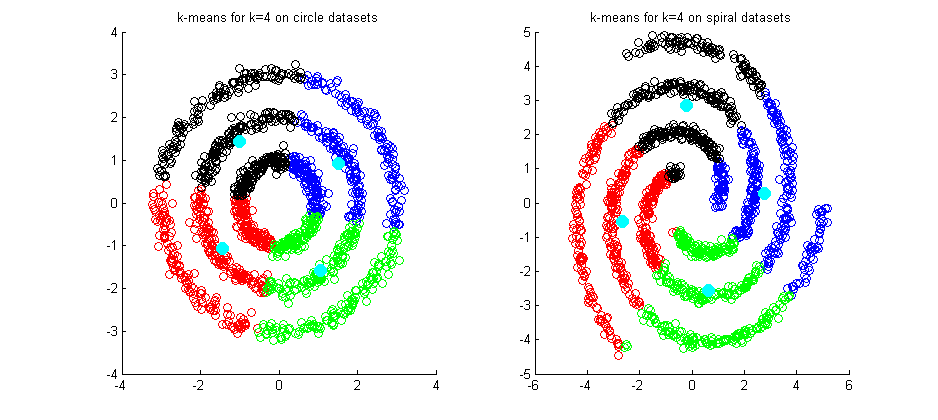
\includegraphics[scale=0.6]{kmeans_k4}
	\\\\\\
	The cyan points in graphs indicate the centroids for each of the clusters. The overall sums of l2 distances between each point and the centroid for the clusters are:
	\\\\
	cluster 1 (red) - circle: 757.41, spiral: 1098.18\\
	cluster 2 (blue) - circle: 721.62, spiral: 1088.39\\
	cluster 3 (green) - circle: 522.01, spiral: 750.26\\
	cluster 4 (black) - circle: 444.34, spiral: 609.27
	\\\\\\
	The eigenvalues of the Laplacian matrices can be seen here:
	\\\\\\
	\hspace*{-3cm}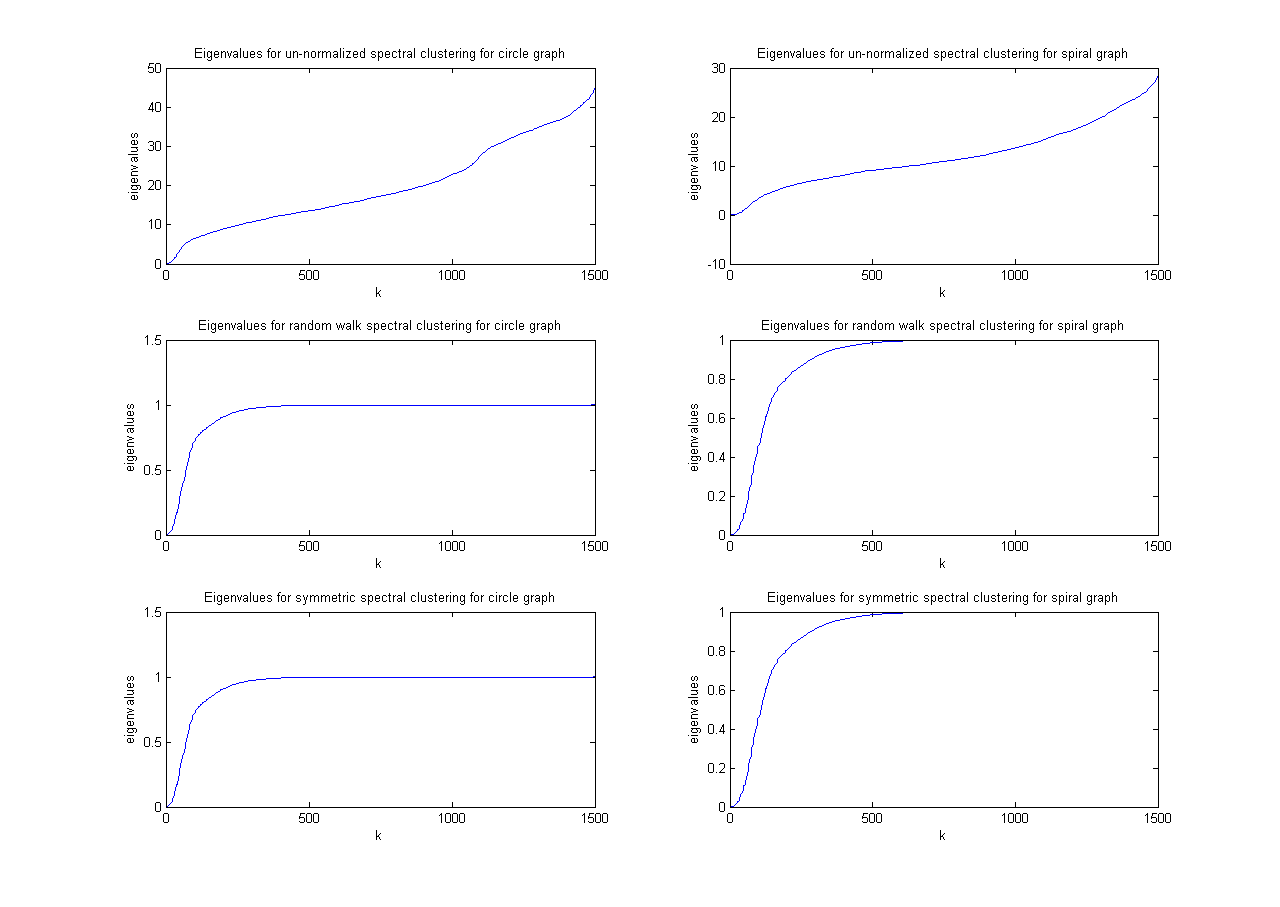
\includegraphics[scale=0.6]{eigenvalues}
	\\\\\\
	After applying spectral clustering we get the following output using symmetric normalization:
	\\\\
	\hspace*{-4cm}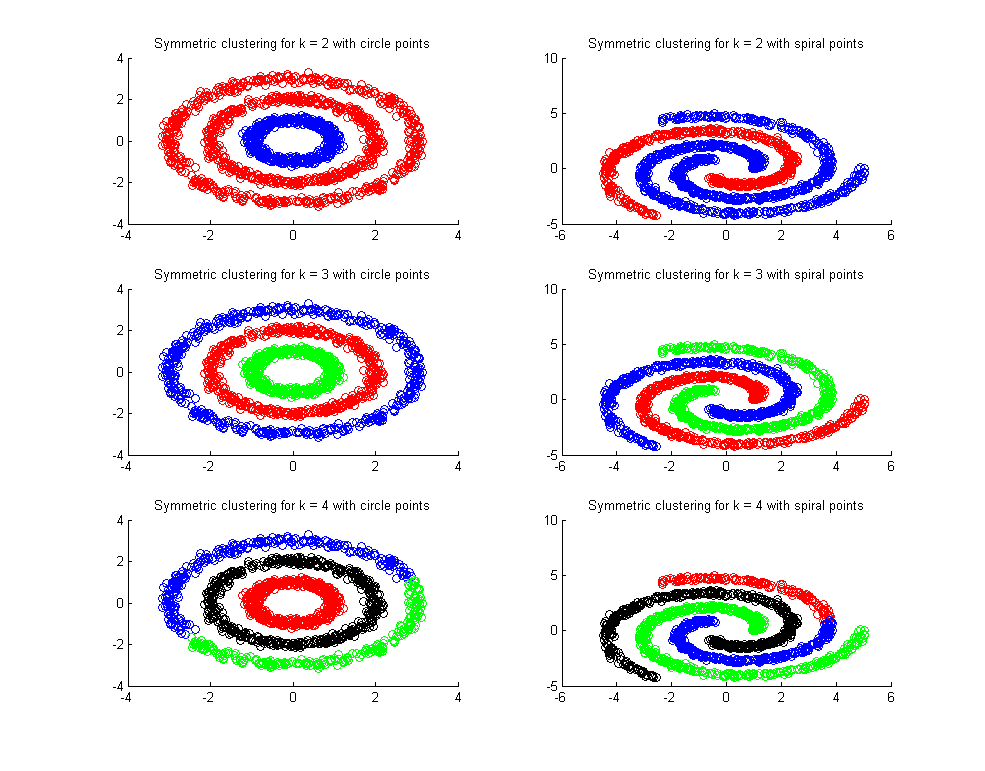
\includegraphics[scale=0.7]{symmetric_spectral_clustering}
	\\\\\\
	In the next figure we can see the 3D interpretation of the eigenvectors, showing that all three clusters are clearly separate in eigenspace:
	\\\\
	\hspace*{-4.3cm}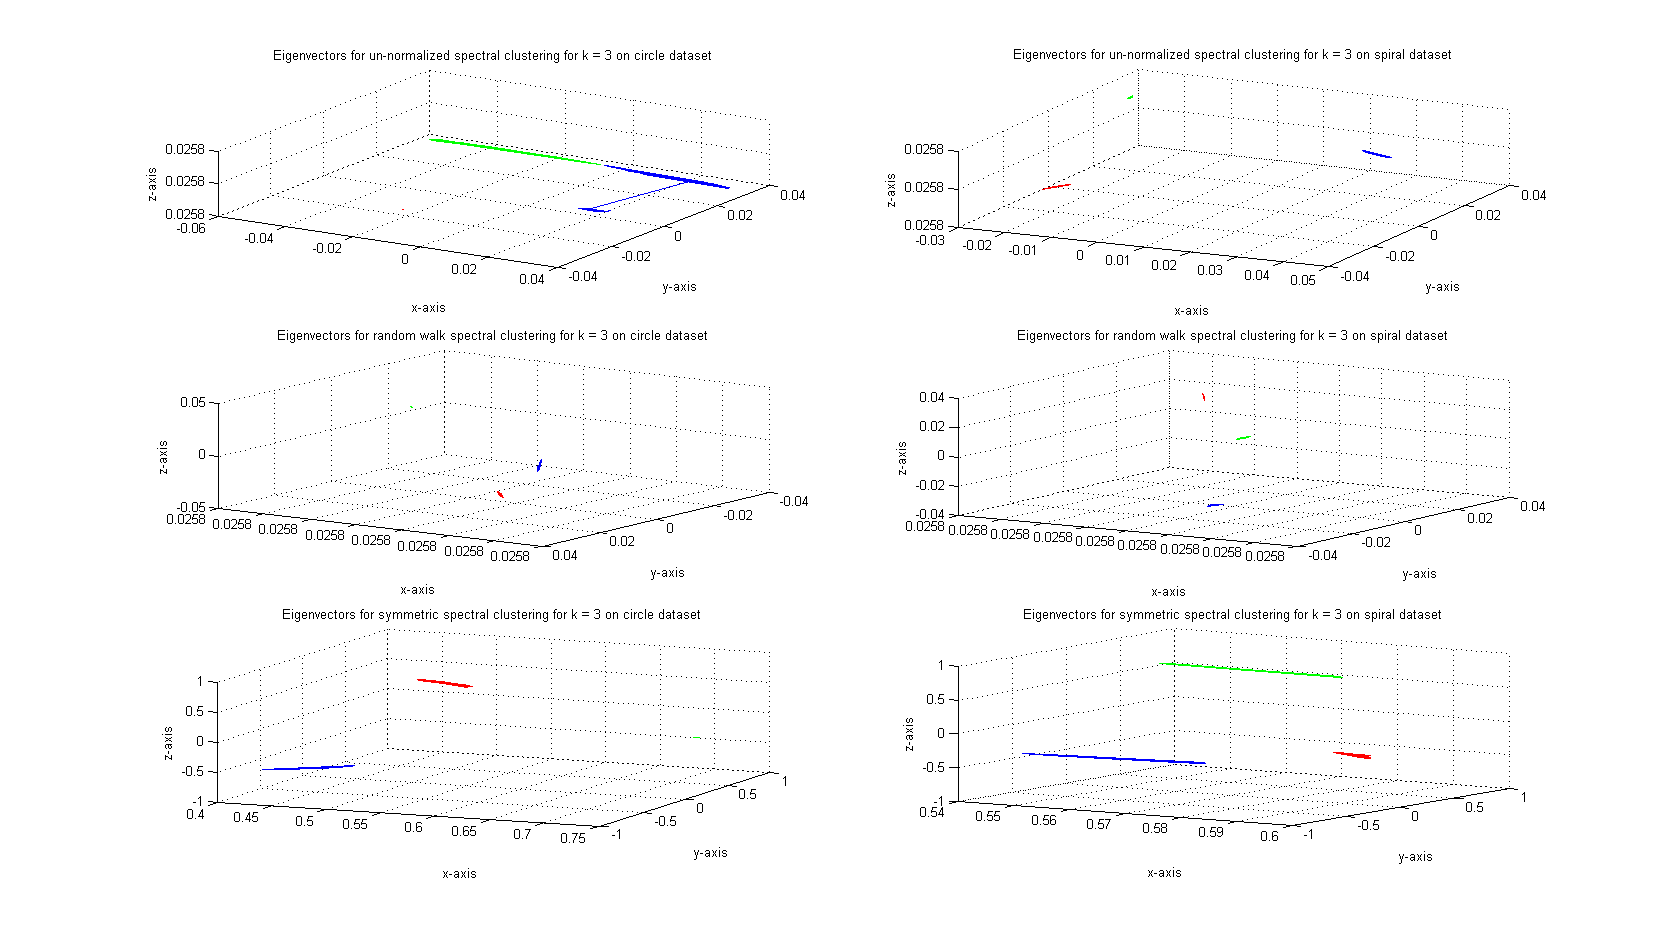
\includegraphics[scale=0.55]{3dplots}
	\\\\\\
	If we convert the data into polar coordinates, we see it is much easier for kmeans to classify the circle dataset, but still difficult to classify the spiral dataset.
	\\\\\\
	\hspace*{-3cm}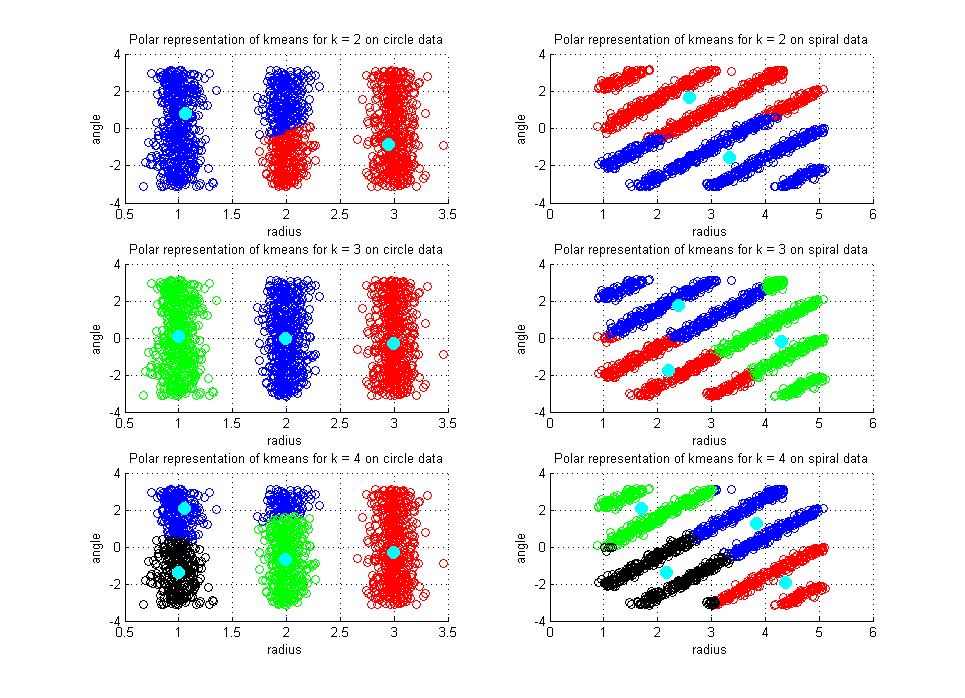
\includegraphics[scale=0.8]{polar_kmeans}
	\\\\\\
	The cyan points in graphs indicate the centroids for each of the clusters. The overall sums of l2 distances between each point and the centroid for the clusters are:
	\\\\
	cluster 1 (red) - circle: 904.57, spiral: 621.46\\
	cluster 2 (blue) - circle: 742.63, spiral: 706.96\\
	cluster 3 (green) - circle: 634.15, spiral: 539.10\\
	cluster 4 (black) - circle: 236.26, spiral: 453.95
	
	\newpage
	\section{Spectral Clustering on Airbnb Data}

	The Purity metric graph can be found here. We can see that we start with very low purity rate when the number of predicted classes is much less than the number of actual classes. As the number of predicted classes rises, so does the purity rate, indicating the clusters are becoming closer to reality.
	\\\\\\
	\hspace*{-1cm}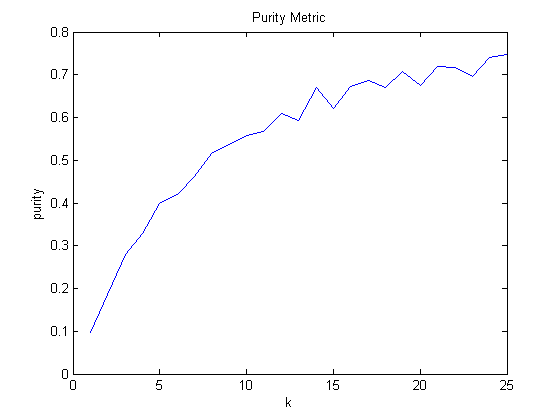
\includegraphics[]{purity}
	\\\\\\
	For k = 5 we can plot the clusters found onto the Google map:
	\\\\
	\hspace*{-1cm}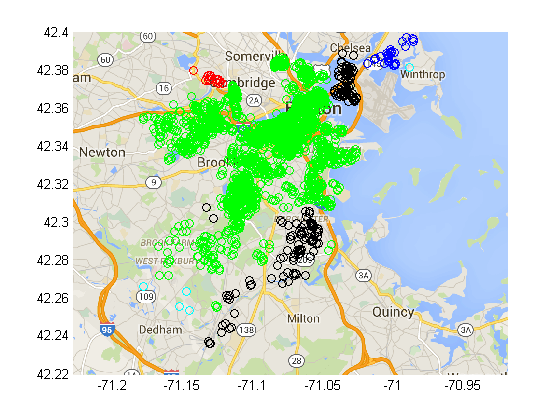
\includegraphics[]{google_map}
%	\\\\\\
%	Using a value of $\sigma=0.01$ is leading to poor results overall. As can be seen from the purity graph, our value doesn't go above 0.5, or half the points are correctly clustered. Further the clusters found for k=5 show that there are large inconsistencies in their distribution. If we switch back to using a $\sigma=0.2$ we get much better results, as indicated below:
%	\\\\\\
%	\hspace*{-1cm}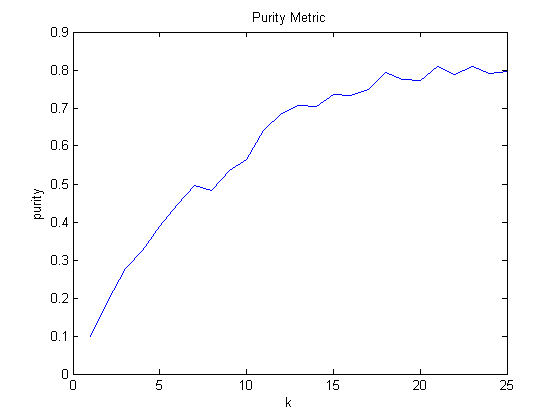
\includegraphics[scale=0.8]{purity_sigma_2}
%	\\\\
%	\hspace*{-1cm}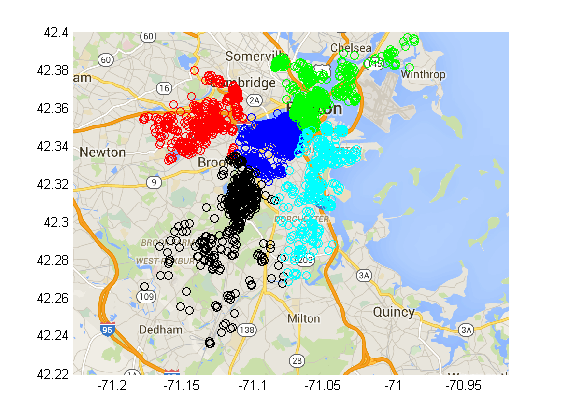
\includegraphics[]{google_map_signa2}
\end{document}